\documentclass[]{article}
\usepackage{lmodern}
\usepackage{amssymb,amsmath}
\usepackage{ifxetex,ifluatex}
\usepackage{fixltx2e} % provides \textsubscript
\ifnum 0\ifxetex 1\fi\ifluatex 1\fi=0 % if pdftex
  \usepackage[T1]{fontenc}
  \usepackage[utf8]{inputenc}
\else % if luatex or xelatex
  \ifxetex
    \usepackage{mathspec}
  \else
    \usepackage{fontspec}
  \fi
  \defaultfontfeatures{Ligatures=TeX,Scale=MatchLowercase}
\fi
% use upquote if available, for straight quotes in verbatim environments
\IfFileExists{upquote.sty}{\usepackage{upquote}}{}
% use microtype if available
\IfFileExists{microtype.sty}{%
\usepackage{microtype}
\UseMicrotypeSet[protrusion]{basicmath} % disable protrusion for tt fonts
}{}
\usepackage[margin=1in]{geometry}
\usepackage{hyperref}
\hypersetup{unicode=true,
            pdftitle={Assignment 1},
            pdfauthor={Per Emil Hammarlund, Albert Öst},
            pdfborder={0 0 0},
            breaklinks=true}
\urlstyle{same}  % don't use monospace font for urls
\usepackage{longtable,booktabs}
\usepackage{graphicx,grffile}
\makeatletter
\def\maxwidth{\ifdim\Gin@nat@width>\linewidth\linewidth\else\Gin@nat@width\fi}
\def\maxheight{\ifdim\Gin@nat@height>\textheight\textheight\else\Gin@nat@height\fi}
\makeatother
% Scale images if necessary, so that they will not overflow the page
% margins by default, and it is still possible to overwrite the defaults
% using explicit options in \includegraphics[width, height, ...]{}
\setkeys{Gin}{width=\maxwidth,height=\maxheight,keepaspectratio}
\IfFileExists{parskip.sty}{%
\usepackage{parskip}
}{% else
\setlength{\parindent}{0pt}
\setlength{\parskip}{6pt plus 2pt minus 1pt}
}
\setlength{\emergencystretch}{3em}  % prevent overfull lines
\providecommand{\tightlist}{%
  \setlength{\itemsep}{0pt}\setlength{\parskip}{0pt}}
\setcounter{secnumdepth}{0}
% Redefines (sub)paragraphs to behave more like sections
\ifx\paragraph\undefined\else
\let\oldparagraph\paragraph
\renewcommand{\paragraph}[1]{\oldparagraph{#1}\mbox{}}
\fi
\ifx\subparagraph\undefined\else
\let\oldsubparagraph\subparagraph
\renewcommand{\subparagraph}[1]{\oldsubparagraph{#1}\mbox{}}
\fi

%%% Use protect on footnotes to avoid problems with footnotes in titles
\let\rmarkdownfootnote\footnote%
\def\footnote{\protect\rmarkdownfootnote}

%%% Change title format to be more compact
\usepackage{titling}

% Create subtitle command for use in maketitle
\providecommand{\subtitle}[1]{
  \posttitle{
    \begin{center}\large#1\end{center}
    }
}

\setlength{\droptitle}{-2em}

  \title{Assignment 1}
    \pretitle{\vspace{\droptitle}\centering\huge}
  \posttitle{\par}
    \author{Per Emil Hammarlund, Albert Öst}
    \preauthor{\centering\large\emph}
  \postauthor{\par}
      \predate{\centering\large\emph}
  \postdate{\par}
    \date{2019-04-15}

\usepackage{float}
\let\origfigure\figure
\let\endorigfigure\endfigure
\renewenvironment{figure}[1][2] {
    \expandafter\origfigure\expandafter[H]
} {
    \endorigfigure
}

\begin{document}
\maketitle

\tableofcontents

\newpage

\hypertarget{exercise-1}{%
\section{Exercise 1}\label{exercise-1}}

For the markov chain:

\[q = \begin{pmatrix} 0.75 \\ 0.25 \end{pmatrix}, A = \begin{pmatrix} 0.99 & 0.01 \\ 0.03 & 0.97\end{pmatrix}\]

The state distribution for the first time step \(t = 1\) is:

\[P(S_1 = 1) = q(1) = 0.75\] \[P(S_1 = 2) = q(2) = 0.25\]

For the second time step \(t = 2\), the distribution of states is:

\[P(S_2 = 1) = \sum_{j = 1}^{2} P(S_1 = j) P(S_2 = 1 | S_1 = j)\]
\[= P(S_1 = 1) P(S_2 = 1 | S_1 = 1) + P(S_1 = 2) P(S_2 = 1 | S_1 = 2)\]
\[= q(1) A(1, 1) + q(2) A(2, 1)  = 0.75 \cdot 0.99 + 0.25 \cdot 0.03 = 0.75\]

\[P(S_2 = 2) = \sum_{j = 1}^{2} P(S_1 = j) P(S_2 = 2 | S_1 = j)\]
\[= P(S_1 = 1) P(S_2 = 2 | S_1 = 1) + P(S_1 = 2) P(S_2 = 2 | S_1 = 2)\]
\[= q(1) A(1, 2) + q(2) A(2, 2) = 0.75 \cdot 0.01 + 0.25 \cdot 0.97 = 0.25\]

Which again, is the same distribution as the first time step. And since
the distribution of a given time step will always be calculated by
marginalizing out the previous time step from the joint
\(P(S_t, S_{t - 1}\) for each of the states in the current time step.
The same calculations will be performed
\(\forall t \in \{ 1, 2, 3, ... \}\) and thus, \(P(S_t = j)\) is
constant for all timesteps.

\newpage

\hypertarget{exercise-2}{%
\section{Exercise 2}\label{exercise-2}}

The distribution of states for \(10 000\) samples from the given markov
chain takes the following form:

\begin{figure}
\centering
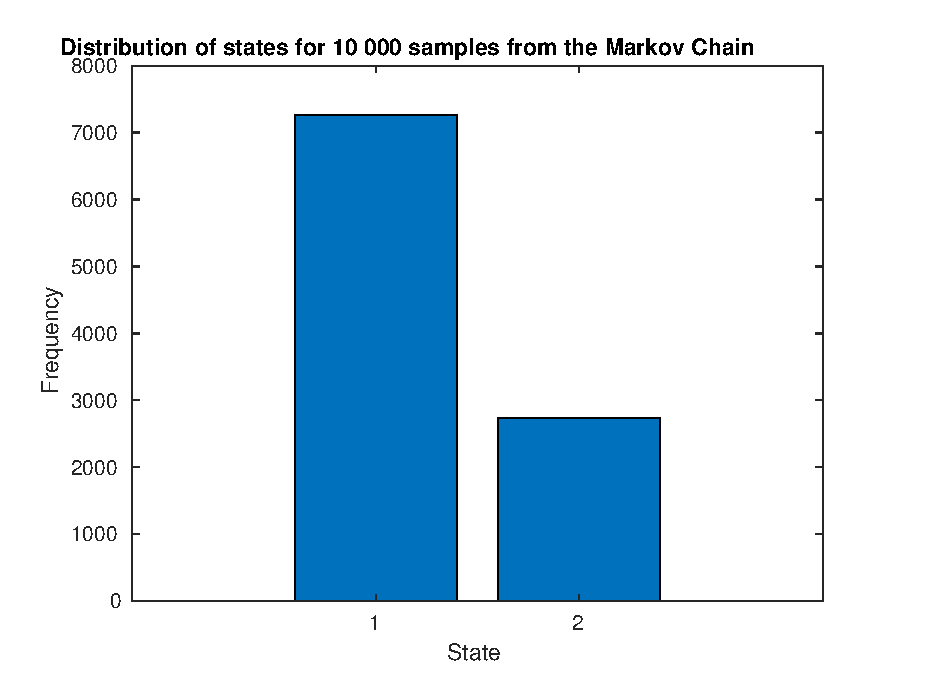
\includegraphics{Result_Pics/stateDistr.eps}
\caption{Distribution of states over 10 000 samples}
\end{figure}

With the frequencies:

\begin{longtable}[]{@{}lll@{}}
\toprule
State & Frequency & Relative Frequency\tabularnewline
\midrule
\endhead
1 & 7265 & 0.7625\tabularnewline
2 & 2735 & 0.2735\tabularnewline
\bottomrule
\end{longtable}

\newpage

\hypertarget{exercise-3}{%
\section{Exercise 3}\label{exercise-3}}

\hypertarget{calculation-of-mathbbex}{%
\subsection{\texorpdfstring{Calculation of
\(\mathbb{E}[X]\)}{Calculation of \textbackslash{}mathbb\{E\}{[}X{]}}}\label{calculation-of-mathbbex}}

\[\mu_X = \mathbb{E} [X] = \mathbb{E}_Z[ \mathbb{E}_X [X | Z]] = \mathbb{E}_Z [ \mathbb{E}_X [b_Z (X)] ] = \sum_{j = 1}^{2} \mathbb{E}_X [X | Z = j] P(Z = j)\]
\[= \mathbb{E}_X [b_1 (x)] P(Z = 1) + \mathbb{E} [b_2 (x)] P(Z = 2)\]
\[=\{\textnormal{since the first order moment of a normal distribution is its mean}\}\]
\[= 0 \cdot 0.75 + 3 \cdot 0.25 = \frac{3}{4}\]

\hypertarget{calculation-of-var_x-x}{%
\subsection{\texorpdfstring{Calculation of
\(var_X [X]\)}{Calculation of var\_X {[}X{]}}}\label{calculation-of-var_x-x}}

\[var[X] = \mathbb{E}_Z[var_X[X | Z]] + var_Z [\mathbb{E}_X[X | Z]] = \mathbb{E}_Z[var_X[X | Z]] + \mathbb{E}_Z [(\mathbb{E}_X [X | Z])^2] - (\mathbb{E}[X])^2\]
\[= \sum_{j = 1}^{2} var_X [X | Z = j] P(Z = j) + \sum_{j = 1}^{2} (\mathbb{E}_X[X | Z = j])^2 P(Z = j) - (\frac{3}{4})^2\]
\[= \sum_{j = 1}^{2} (var_X [X | Z = j] + (\mathbb{E}_X[X | Z = j])^2) P(Z = j) - (\frac{3}{4})^2\]
\[= (var_X [X | Z = 1] + (\mathbb{E}_X[X | Z = 1])^2) P(Z = 1) + (var_X [X | Z = 2] + (\mathbb{E}_X[X | Z = 2])^2) P(Z = 2) - \frac{9}{16}\]
\[= (1 + 0^2) \cdot 0.75 + (4 + 9) \cdot 0.25 - \frac{9}{16} = \frac{3}{4} + \frac{13}{4} - \frac{9}{16} = \frac{12}{16} + \frac{52}{16} - \frac{9}{16} = \frac{55}{16} = 3.4375\]

\hypertarget{verification-of-implemented-code}{%
\subsection{Verification of implemented
code}\label{verification-of-implemented-code}}

When generating 10 000 samples from the HMM rand function, the following
mean and variance was observed:

\begin{longtable}[]{@{}ll@{}}
\toprule
mean & variance\tabularnewline
\midrule
\endhead
0.7831 & 3.5241\tabularnewline
\bottomrule
\end{longtable}

\newpage

\hypertarget{exercise-4}{%
\section{Exercise 4}\label{exercise-4}}

The samples from 500 contiguous samples \(X_t\) took the following form:

\begin{figure}
\centering
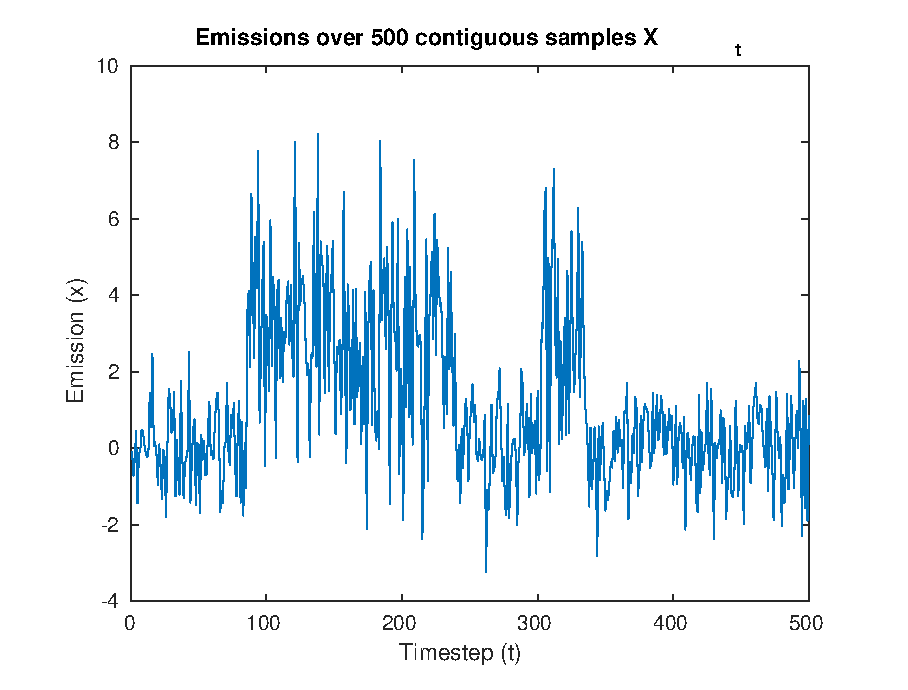
\includegraphics{Result_Pics/emissionDistr.eps}
\caption{Samples from 500 contiguous samples from the hmm rand function}
\end{figure}

As can be seen in figure 2 above, the distribution that is generating
emissions from the hidden markov model (i.e.~the hidden state) tends to
stick in the same hidden state rather then transition between the
states. This makes sense since staying in the same hidden state is far
more likely then transitioning.

\newpage

\hypertarget{exercise-5}{%
\section{Exercise 5}\label{exercise-5}}

The observed emissions from the hidden markov model took the following
form:

\begin{figure}
\centering
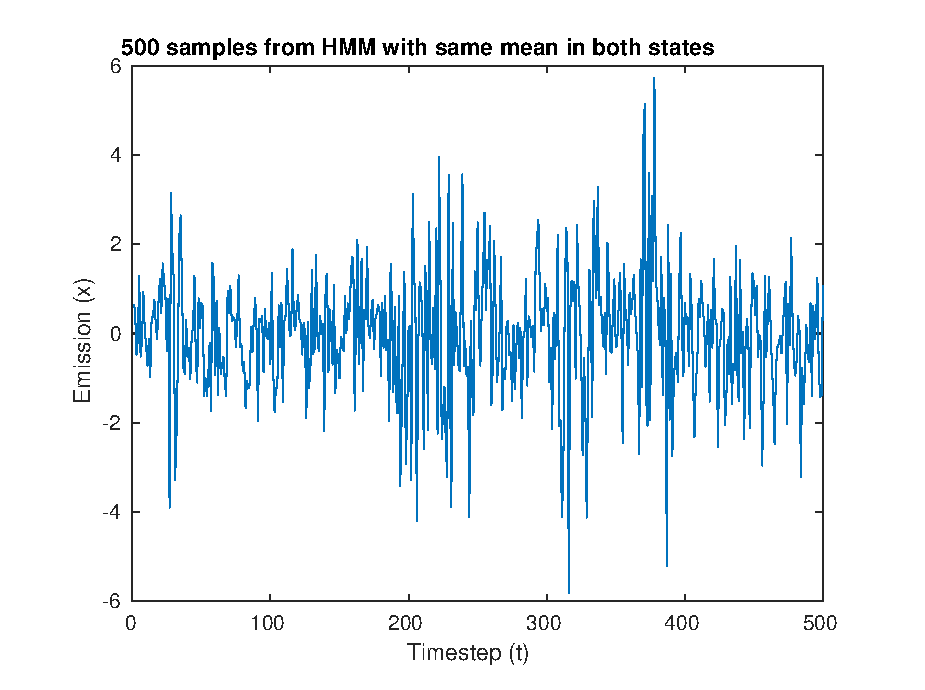
\includegraphics{Result_Pics/emissionDistrEqual.eps}
\caption{Samples from HMM with \(\mu_1 = \mu_2 = 0\)}
\end{figure}

As can be seen in figure 3 above, it is much more difficult to
differentiate the transition between the two distributions and thus by
extension know what hidden state the observations are coming from. It is
of coarse, possible to approximate what hidden states have generated the
emissions, but due to the similarity between the two distributions. It
will not be as accurate.

\newpage

\hypertarget{exercise-6}{%
\section{Exercise 6}\label{exercise-6}}

The finite hidden markov model which can be found in equation 5.17 in
the course book was constructed using the following code:

\begin{verbatim}
mc = MarkovChain([1 ;0], [0.7 0.25 0.05; 0.1 0.8 0.1])
h = HMM(mc, [GaussD('Mean', 0, 'StDev', 1), GaussD('Mean', 3, 'StDev', 2)])
\end{verbatim}

And the rand function was queried for 500 samples 10 000 times and the
length of the observation sequence was saved for each try using:

\begin{verbatim}
num_obs = zeros(10000, 1);
for i=1:10000
    num_obs(i) = size(h.rand(500), 2);
end
fprintf(sprintf('The observations sequence had an average length of %f.\n', mean(num_obs)));
\end{verbatim}

Which gave an average length of \(12.886700\).

This was then compared to the distribution of the expected length of
observations generated from the code below:

\begin{verbatim}
lenDistr = zeros(100, 1);
for i=1:100
lenDistr(i) = sum(mc.InitialProb' * mc.TransitionProb(:, 1:2)^i) * i;
end
lenDistr = lenDistr ./ sum(lenDistr);
plot(lenDistr);
hold on
xlabel('Number of timesteps in transeint states');
ylabel('Probability');
title('Distribution over first 100 timesteps of expected sequence length');
hold off
\end{verbatim}

The distribution of the expected length of the observation sequence
generated from the code above took the following form:

\begin{figure}
\centering
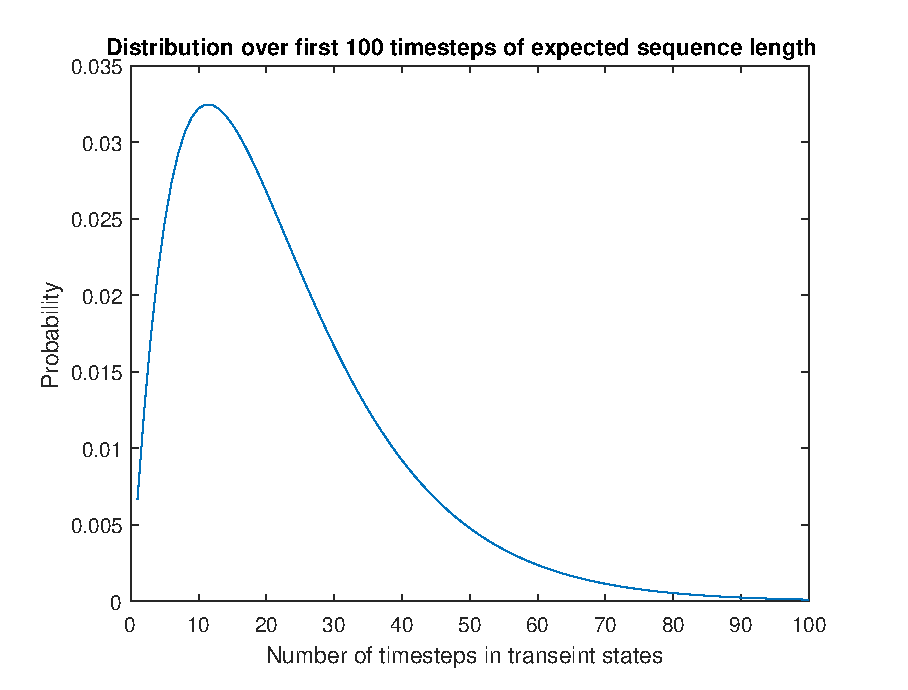
\includegraphics{Result_Pics/lenDistr.eps}
\caption{Distribution of expected sequence length}
\end{figure}

From which it can be observed that the highest density is around 12-13,
which is in the same neighborhood as our average sequence length.

\newpage

\hypertarget{exercise-7}{%
\section{Exercise 7}\label{exercise-7}}

The following hidden markov model was constructed:

\begin{verbatim}
g1 = GaussD('Mean', [3; 3], 'Covariance', [0.01 0; 0 0.01]);
g2 = GaussD('Mean', [0; 0], 'Covariance', [0.01 0.01; 0.01 0.01]);
mc = MarkovChain([0.75; 0.25], [0.99 0.01; 0.03 0.97]);
h = HMM(mc, [g1, g2]);
\end{verbatim}

And 100 samples was drawn from it and visualized using the following
code:

\begin{verbatim}
h = HMM(mc, [g1, g2]);
emissions = h.rand(1000000);
hist3(emissions', 'CdataMode', 'auto', 'Nbins', [100, 100]);
view(2);
colorbar;
hold on
xlabel('dimension 1');
ylabel('dimension 2');
title('Visualisation of emissions from HMM');
hold off
\end{verbatim}

the distribution took the following form:

\begin{figure}
\centering
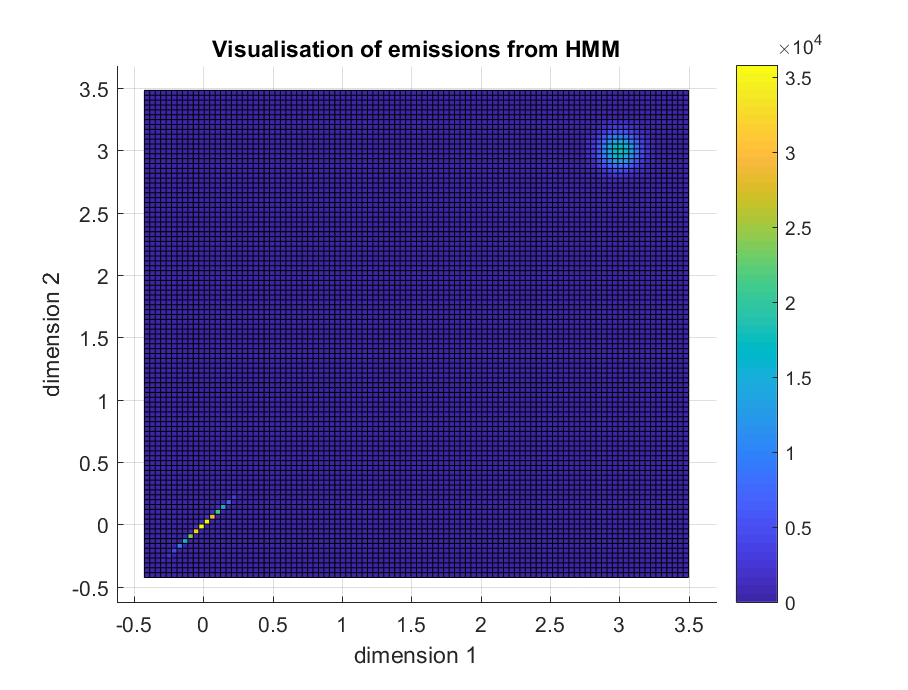
\includegraphics{Result_Pics/emissionMultVar.eps}
\caption{100 samples from HMM with multivariate gaussian distributions}
\end{figure}

From which it is clear that distribution 1 has no correlation between
dimentsions and that distribution 2 has a strong correlation between
dimensions.


\end{document}
